\usepackage{booktabs}%! Author = lazza
%! Date = 11/04/2022

\section{Pipelining}\label{sec:pipeline}

MIPS instructions
\subsection{MIPS}\label{subsec:heterogeneous-systems}
The MIPS architecture is based on the SIMD model.
\begin{figure}
    \centering
    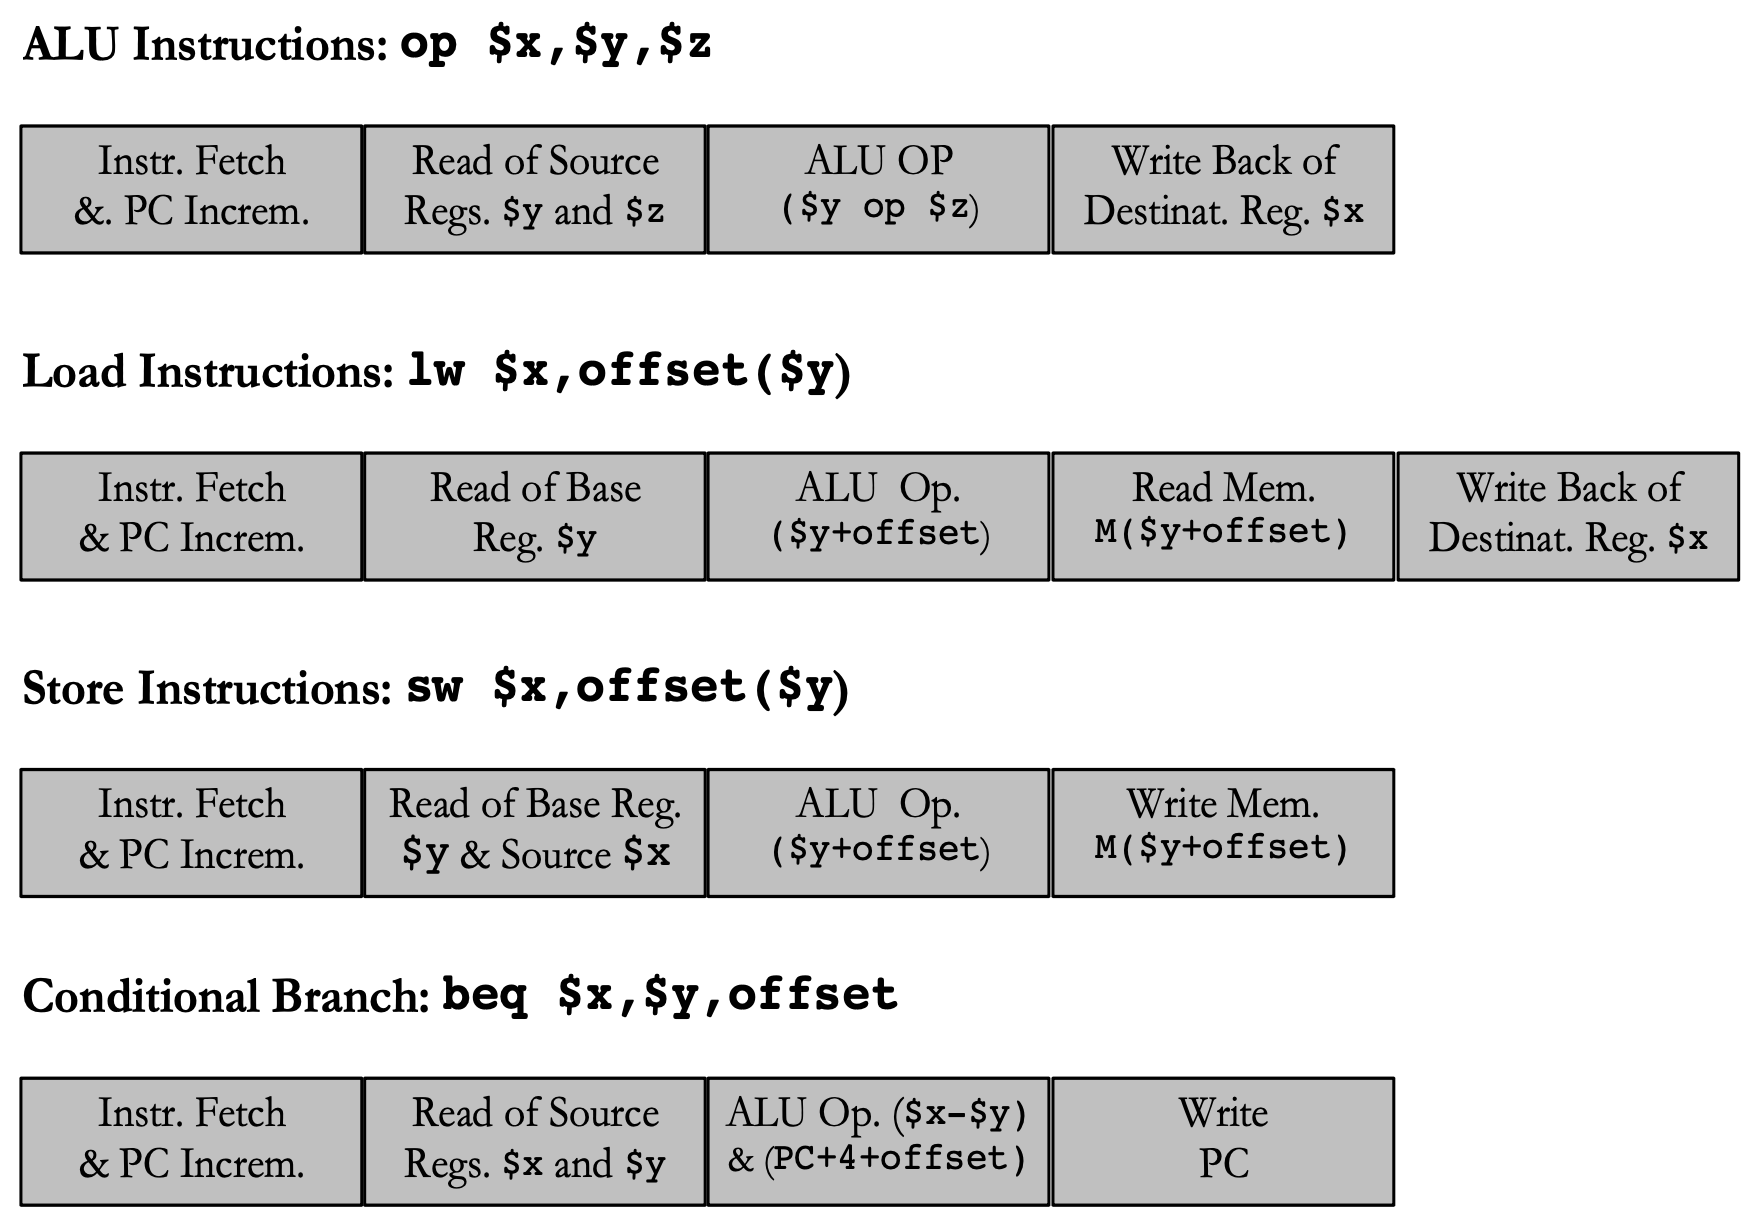
\includegraphics{images/MIPS-instructions}
    \caption{MIPS instructions}
    \label{fig: MIPS instructions}
\end{figure}
Instruction set, 32 bit
architecture specific

Exam:
- assembly --> specific instruction for an architecture
- design architecture

CPU = data path plus  control unit
Bus:
- control
- data
- address
Memory

pipeline multi-cycle process: latency vs throughput

RF : Register file is used in ID and WB phase, clock divided in rising edges and falling edge, sometimes there
are dependencies among instructions

Register File used in 2 stages: Read access during ID and write access during WB
– What happens if read and write refer to the same register in the same clock cycle?
• It is necessary to insert one stall
• OptimizedPipeline:the RF read occurs in the second half of clock cycle and the RF write in the first half of clock
cycle
– What happens if read and write refer to the same register in the same clock cycle?
• It is not necessary to insert one stall

\subsection{Hazards}\label{subsec:hazards}
A hazard is created whenever there is a dependence between instructions, and instructions are close enough that the
overlap caused by pipelining would change the order of access to the operands involved in the dependence.
Hazards prevent the next instruction in the pipeline from executing during its designated clock cycle.
Hazards reduce the performance fromthe ideal speedup gained by pipelining.

\subsubsection{Structural hazards}
Use of the same resource from different instruction simultaneously.
No structural hazards in MIPS architecture:
– Instruction Memory separated from Data Memory
– Register File used in the same clock cycle: Read access by an instruction and write access by another instruction

\subsubsection{Data Hazard}
Attempt to use a result before it is ready

-RAW
Techniques: design (compilation-time) and hardware solutions (run-time)

Compilation Techniques:
– Insertion of nop (no operation) instructions
– Instructions Scheduling to avoid that correlating instructions are too close
    • The compiler tries to insert independent instructions among correlating instructions
    • When the compiler does not find independent instructions, it insert nops.
Hardware Techniques:
– Insertion of “bubbles” or stalls in the pipeline
– Data Forwarding or Bypassing

insertion of nops (no operation), compiler
insertion of bubbles, architecture

scheduling, reordering instruction without changing the overall result

forwarding, shortcutting data from origin to next use EX-EX path, MEM-EX path, MEM-ID path, in WB-ID there's no
need for a path, just persistence trough clock cycle.

-Load/Use hazard, it requires a stall to use the MEM-EX path, two stalls to use the optimized pipelining

-Load/Store hazard, forwarding MEM-WB

MEM-ID path is not useful if we divide clock cycle in rising and falling edge

Other architecture different from 5 stage mips:
-WAW write after write , conflict if write after write are not executed in order
-WAR write after read

Data hazards: RAW(dependency), WAW, WAR(anti-dependency)
immagine slide 17 introilp_v2

\subsubsection{Control hazards}
Attempt to make a decision on the next instruction to execute before the condition is evaluated.
Mux output based on ALU output.
Until alu doesn't compute output PC is not known, we cant know the next instruction.

PC available at the memory stage.

Generally true statements are executed during the waiting for the next instruction, as if the condition is true, just PC plus 1, and then see if the branch is taken.

branch stall with and without forwarding, 3 vs 2 stalls

additional solution is the early evaluation of the PC, new pipeline in witch PC adder is anticipated in the ID stage, 1
stall to fetch the correct instruction

This solution bring an issue with RAW: we do have to insert a stall.

Branch prediction techniques
- static (compile-time)
branch always not taken, no jump
branch always taken, always jump, not always good because we have to calculate BTA branch target address (Mips pipeline)
backward taken forward not taken, loop taken, if not taken
profile-driven prediction, we are going make several runs of our program and the choice is based on statistical data
delayed branch, rescheduling an independent instruction (also from the branch):
    from before (no penalty in mips)
    from target
    from fall-through


- dynamic (run-time)
Branch outcome predictor, to predict the direction of a branch (i.e., taken or not taken).
save the outcome value, i.e,

Branch target predictor, to predict the branch target address in case of taken branch
Save BTA info in a target buffer that  we will use if we take the branch, save the target address.


Branch History Table (or Branch Prediction Buffer) - outcome predictor
Table containing n-bit for each entry that says whether the branch was recently taken or not.
Table indexed by the lower portion of the address of the branch instruction.
slide 11:
n-bits branch store address
k-bits to index the branch addresses in the buffer, 2^k entries
last k-bits of branch store address may collide!

1-bit branch history table
1-bit for each entry says whether the branch was recently taken or not.
Till now we have a profile driven prediction, dynamic element is the update the value based on past instruction
Example:
0, prediction not taken, outcome not taken - no update
0, prediction not taken, outcome taken - update 0 to 1
0, prediction taken, outcome not taken - update 1 to 0
see automata slide 28

A misprediction occurs when:
– The prediction is incorrect for that branch, or
– The same index has been referenced by two different branches, and the previous history refers to the other branch.
    • To solve this problem it is enough to increase the number of rows in the BHT or to use a hashing function (such as in GShare).

2-bit branch history table
The prediction must miss twice before it is changed.
In a loop branch, at the last loop iteration,we do not need to change the prediction.
For each index in the table, the 2-bits are used to encode the four states of a finite state machine.
see automata, 4 states, 2 bits
do exercise slide 74

n-bit branch history tables
best one is 2-bit

correlating branch predictors
(m,n), best one is (2,2)



\section{Exercise session 1 - Data Hazards}\label{sec:exercise-session-1}
IF instruction fetch - ID instruction decode - EX execution - MEM memory access - WB write back

single fetch per clock cycle : Microprocessor without Interlocked Pipelined Stages (SIMD)

data conflict vs data hazards?
A conflict can be an hazard

exercise1:
- highlight conflicts
- data path, introduce forwarding, memorize data path + 3 forwarding path (diagonal) + 1 forwarding in the same clock
- rescheduling

exercise2:
- highlight conflicts
Resolve data hazards
- without forwarding, stalls
- with forwarding
- scheduling
Resolve control hazards
- apply backward taken forward not taken

Problem:
solution a
\[CPI = \frac{clock cycles}{instruction} = \sum_{i=0}^{n} CPI_i \times F_i\]
where \(F_i = \frac{I_i}{Instruction count}\)

solution b,c,d vedo formulario


\section{Exercise session 2}\label{sec:exercise-session-2}
Performance analysis

Throughput vs Response time (latency?)
- faster hardware : more throughput and minor response time
- adding parallel hardware: more throughput

Amdahl's law
1) Hardware : Enhance fraction (of our application, program), if we enhance the entire application the max overall
speedup is = 2,86.

2)Parallelism: strong scaling, #thread vs serial part of a program
Power consumption?

3) pipelining
conflict = dependency != hazard

4) dynamic branch prediction


\section{Instruction level parallelism}\label{sec:instruction-level-parallelism}
Definition: potential overlap of execution among unrelated instructions
Overlapping possible if:
- no structural hazards
- no raw, war, waw stalls
- no control hazards

pipeline CPI

In mips the only possible structural hazards is WB-ID where the same resource/register can be accessed,
this issued is solved diving the clock cycle in rising edge (WB) and falling edge (ID).

WAR and WAW were not possible with ADD operation with integers, MULT and DIV use floating point numbers.
New stage introduced, it allows for multi-cycloes - complex pipelining, problem synchronization, out-of-order write
hazards due to variable latencies of different FUs.

WB-ISSUE same cycle instead of WB-ID\@.
Mulitple arrows entering the WB, variable latency can cause concurrent writes (besides out-of-order writes).

all functional units are pipelined!

learn assumptions<<

dependencies:
- data
- control
- name, WAR & WAW generated by the lack of registers

Techniques:
--> renaming
--> scheduling: static (compiler) and dynamic

-> superscalar


